\chapter{The Optimal Games}\label{ch:opt}

In the previous chapters various aspects of the different language games have been investigated. Chapter \ref{ch:basic} introduced the basic experiment. Variations that have been investigated in chapter \ref{ch:lex} indicated some possible improvements on the basic model. This chapter combines some proposed improvements in the most interesting language games: the guessing game and the observational game.

The first set of experiments that will be investigated involves the {\em guessing game}. Although not most successful at first sight, the guessing game scenario is an important scenario that is also applied in the Talking Heads experiment. To enable a fruitful discussion with the Talking Heads experiments, this scenario is investigated first and in most detail. This experiment is investigated in section \ref{s:opt:gg}.

The observational language game is explored as a second experiment in section \ref{s:opt:oli}. The results of this experiment in the previous chapter were very promising, and it is possibly a very common strategy in language development.


  Instead of doing 10 runs of 5,000 language games, each experiment is done with 10 runs of 10,000 language games. This will make it harder to compare these experiments with previous experiments. On the other hand the resulting systems can be investigated more reliably, because many systems were still learning after 5,000 games. 


\section{The Guessing Game}\label{s:opt:gg}
\index{guessing game|(}

\subsection{The Experiments}

The two experiments presented in this section implement the guessing game. The basic experiment has been optimised by changing the following strategies and parameters:

\begin{itemize}
\item The categorisation is unaltered, i.e. the prototype method is used, because no drastic improvements have been observed in the other methods and the implemented method is relatively fast.

\item The physical interaction is improved by applying new gearing on the robots. Although the differences were not very significant, the results were better than the basic data set.

\item The creation probability is set to $P_s=0.4$ in one experiment (P.4) and $P_s=0.1$ in another (P.1), because these values revealed most promising results in section \ref{s:par:ps}.

\item Learning rate $\eta$ is set to $\eta-0.9$. A value that holds a relatively long history of interactions. It allows sufficiently fast learning.

\item Word-forms are adopted under all proposed circumstances. I.e. when novel word-forms are encountered, or the matching meaning does not match the relevant topic. The topic with which the form is adopted is selected at random, since no overt differences have been observed in the experiments of section \ref{s:par:adopt}.
\end{itemize}


\begin{table}
\centering
\begin{tabular}{cc}
\lsptoprule
Type of change & Value\\\midrule
Data-set & new gearing\\%\hline
$P_s$ & 0.1 and 0.4\\%\hline
$\eta$ & 0.9\\%\hline
Adoption strategy & random\\%\hline
\lspbottomrule
\end{tabular}
\caption{The set-up of the optimal guessing game.}
\label{t:opt:gg1}
\end{table}

The differences are summarised in table \ref{t:opt:gg1}. Instead of 10 runs of 5,000 games, 10 runs of 10,000 games are played. The two experiments of this section are now defined as above with the two variants:

\begin{description}
\item[P.1] Word-form creation probability $P_s=0.1$.
\item[P.4] Word-form creation probability $P_s=0.4$.
\end{description}


\subsection{The Results}

The experiments are done with 10 runs of 10,000 guessing games. Figures \ref{f:opt:ggplotsp.1} and \ref{f:opt:ggplots} show the evolution of the qualitative measures and the averaged results of both experiments are shown in table \ref{t:opt:ggavg}. The two experiments are qualitatively very much the same. Except the specificity differs from each other significantly $p=0.0000$. The specificity in experiment P.1 is 0.075 higher as in the basic experiment ($p=0.0000$). In P.4 the specificity is even 0.12 higher. As discussed in the previous chapter, the higher specificity has to do with the higher $P_s$. When comparing the evolutions of the specificity in figures \ref{f:opt:ggplotsp.1} (c) and \ref{f:opt:ggplots} (c), it is clear that the specificity in experiment P.1 is still increasing towards the end. So the difference becomes less near the end.

Clearly the communicative success approaches the potential understandability of 80 \% in both experiments. After 10,000 games, the CS is approximately 75 \% on the average. The discriminative success is on the average about 97 \%, thus approaching 100 \% at the end of the experiment. On the average the distinctiveness is about 0.02 higher than in the basic experiment. Parsimony is only a little higher than in the basic experiment (0.861 vs. 0.851). Consistency is about 0.045 higher than in the basic experiment. All these differences have a significance of $p=0.0000$.

\begin{figure}
\centering
\subfigure[CS]{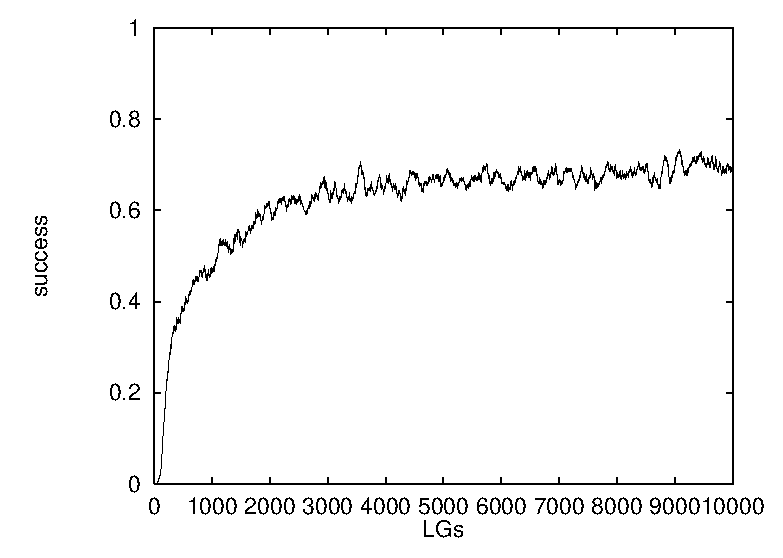
\includegraphics[width=5.5cm]{optimal/csoptp.eps}}
\subfigure[DS]{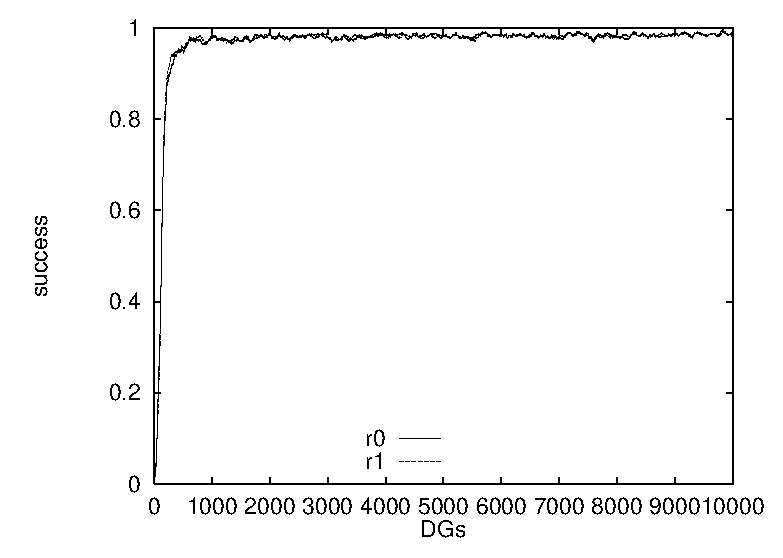
\includegraphics[width=5.5cm]{optimal/dsoptp.eps}}\\
\subfigure[S]{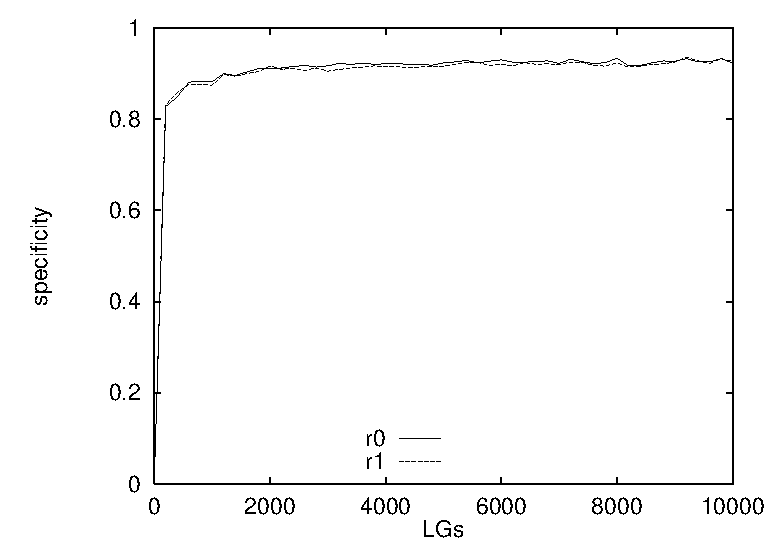
\includegraphics[width=5.5cm]{optimal/soptp.eps}}
\subfigure[D]{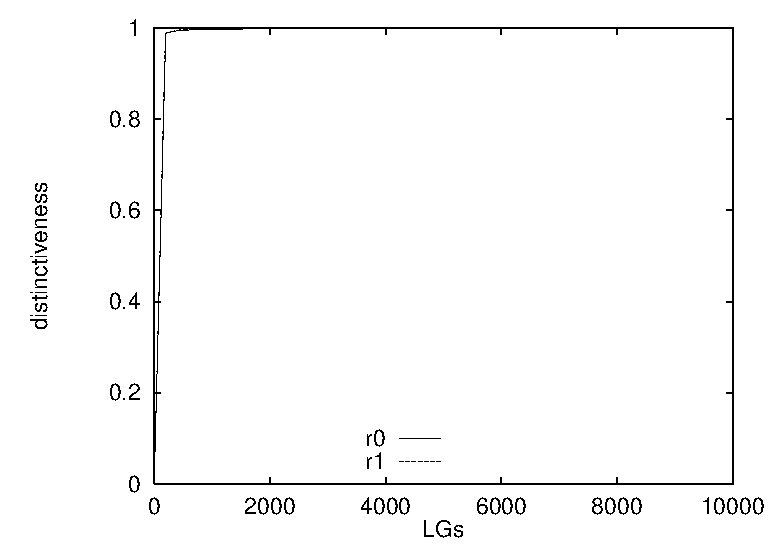
\includegraphics[width=5.5cm]{optimal/doptp.eps}}\\
\subfigure[C]{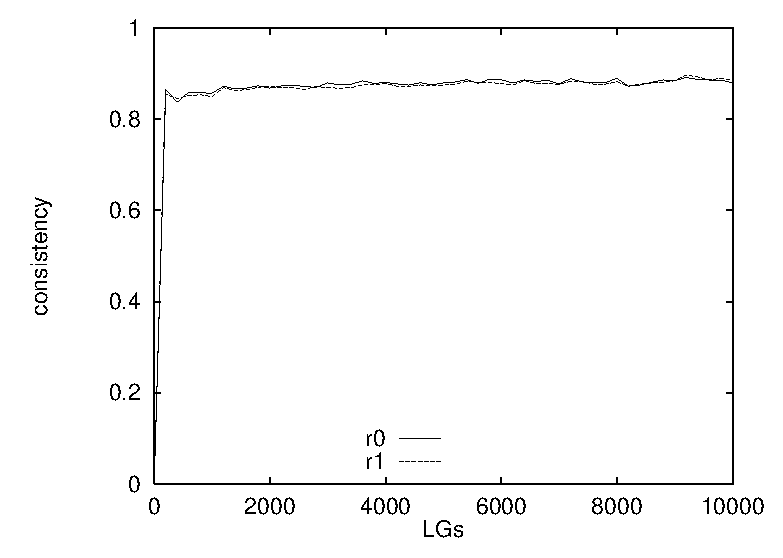
\includegraphics[width=5.5cm]{optimal/coptp.eps}}
\subfigure[P]{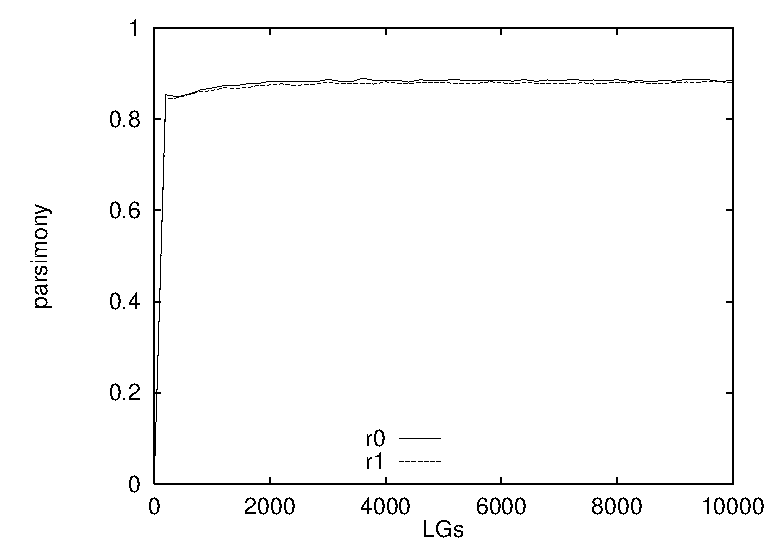
\includegraphics[width=5.5cm]{optimal/poptp.eps}}
\caption{The evolution of the optimal guessing game experiment P.1.}
\label{f:opt:ggplotsp.1}
\end{figure}

\begin{figure}
\centering
\subfigure[CS]{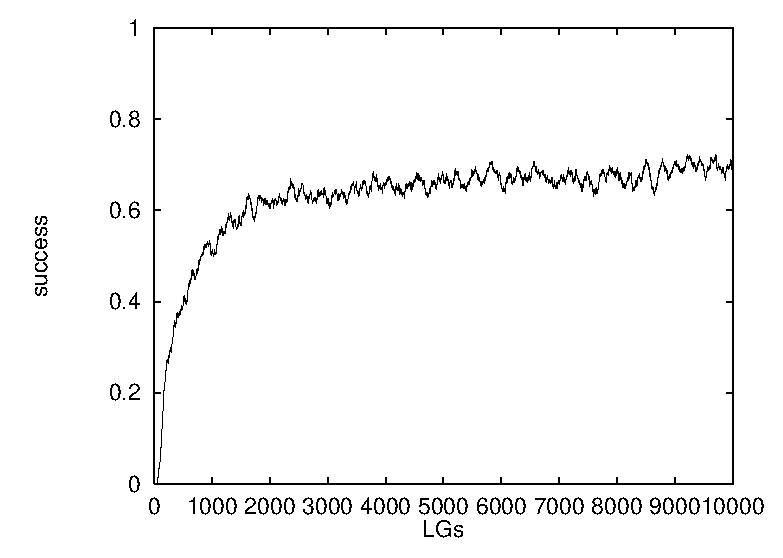
\includegraphics[width=5.5cm]{optimal/csopt.eps}}
\subfigure[DS]{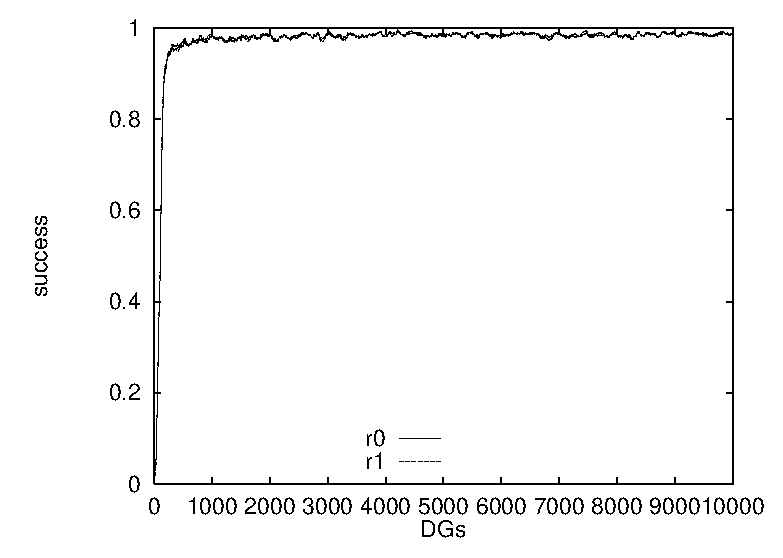
\includegraphics[width=5.5cm]{optimal/dsopt.eps}}\\
\subfigure[S]{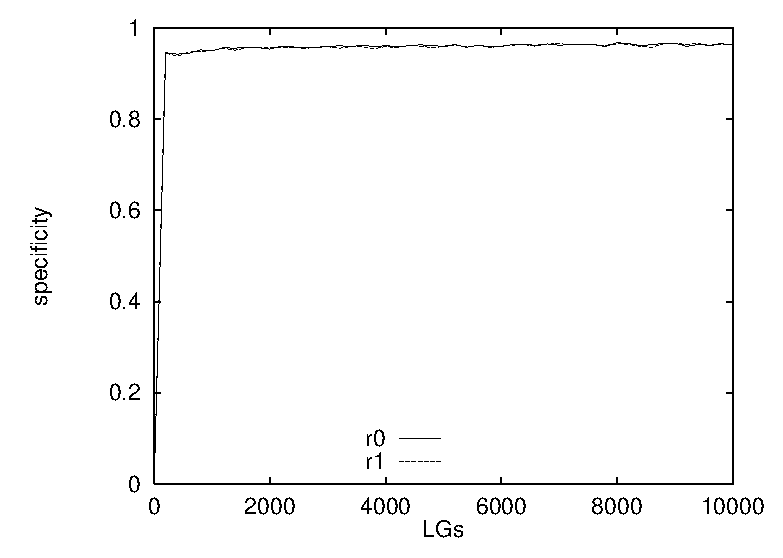
\includegraphics[width=5.5cm]{optimal/sopt.eps}}
\subfigure[D]{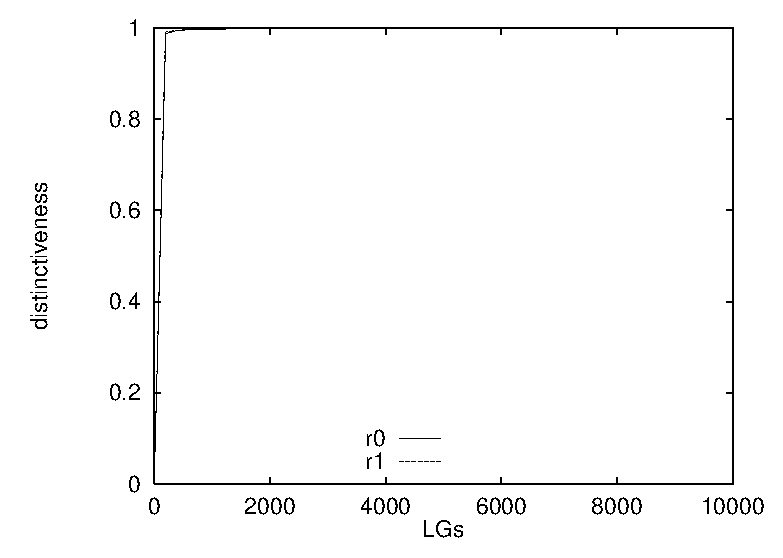
\includegraphics[width=5.5cm]{optimal/dopt.eps}}\\
\subfigure[C]{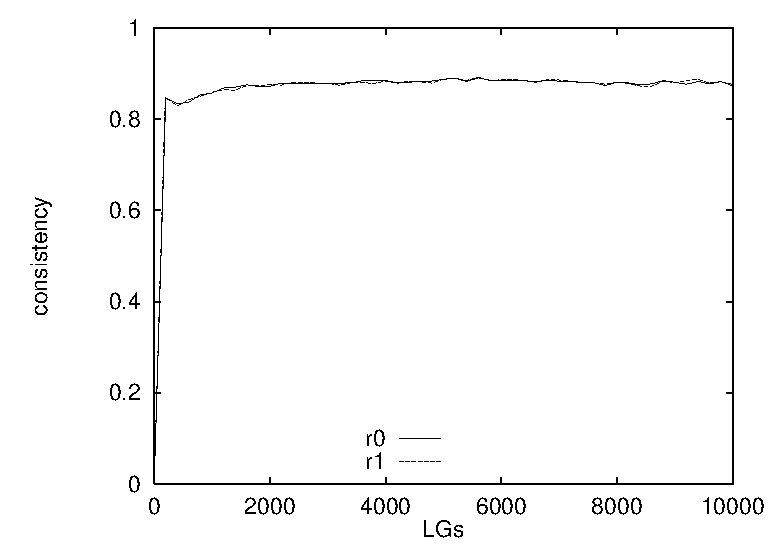
\includegraphics[width=5.5cm]{optimal/copt.eps}}
\subfigure[P]{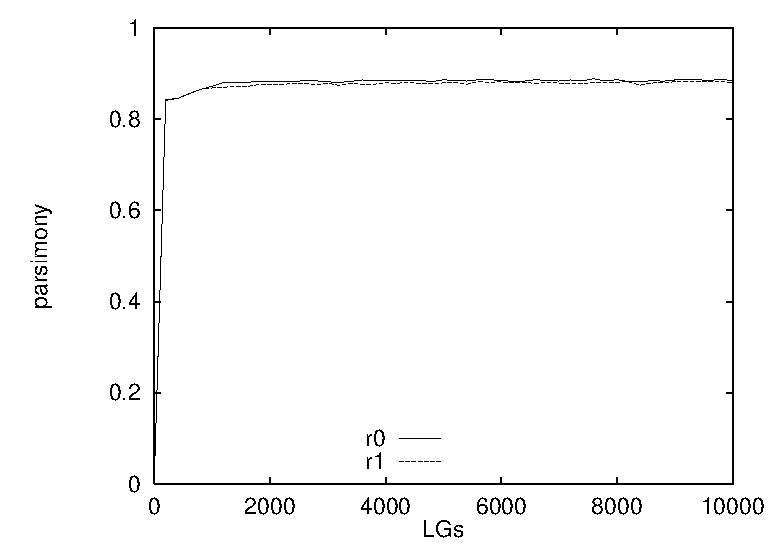
\includegraphics[width=5.5cm]{optimal/popt.eps}}
\caption{The evolution of the optimal guessing game experiment P.4. }
\label{f:opt:ggplots}
\end{figure}

\begin{table}
\centering
\begin{tabular}{lcc}
\lsptoprule
Score & P.1 & P.4 \\\midrule
CS & 0.624$\pm$0.008& 0.628$\pm$0.001\\%\hline
DS0 & 0.972$\pm$0.001 & 0.976$\pm$0.001\\%\hline
DS1 & 0.972$\pm$0.001 & 0.977$\pm$0.001\\%\hline
D0 & 0.979$\pm$0.000 & 0.979$\pm$0.000\\%\hline
D1 & 0.979$\pm$0.000 & 0.979$\pm$0.000\\%\hline
P0 & 0.864$\pm$0.001 & 0.864$\pm$0.001\\%\hline
P1& 0.859$\pm$0.000 & 0.859$\pm$0.000\\%\hline
S0 & 0.898$\pm$0.005 & 0.941$\pm$0.002\\%\hline
S1 & 0.894$\pm$0.005 & 0.940$\pm$0.003\\%\hline
C0 & 0.860$\pm$0.001 & 0.860$\pm$0.002\\%\hline
C1 & 0.857$\pm$0.002 & 0.860$\pm$0.001\\%\hline
\lspbottomrule
\end{tabular}
\caption{The averaged results of the optimal guessing game experiment.}
\label{t:opt:ggavg}
\end{table}

So, the system finally becomes very good in constructing a lexicon by which the robots can communicate about the things they detect in their environment.

\index{semiotic landscape|(}
The run that will be discussed in more detail below resulted in the lexicon that is displayed in the semiotic landscape shown in figure \ref{f:opt:semiotic} and is taken from experiment P.1. This figure shows the connections with a strength that represents the frequency of connections that are successfully used. Ideally, the connections between referent-form-referent would be orthogonal. I.e. the couplings of a referent and its form should not cross-connect with other referents.

\begin{figure}[t]
\centerline{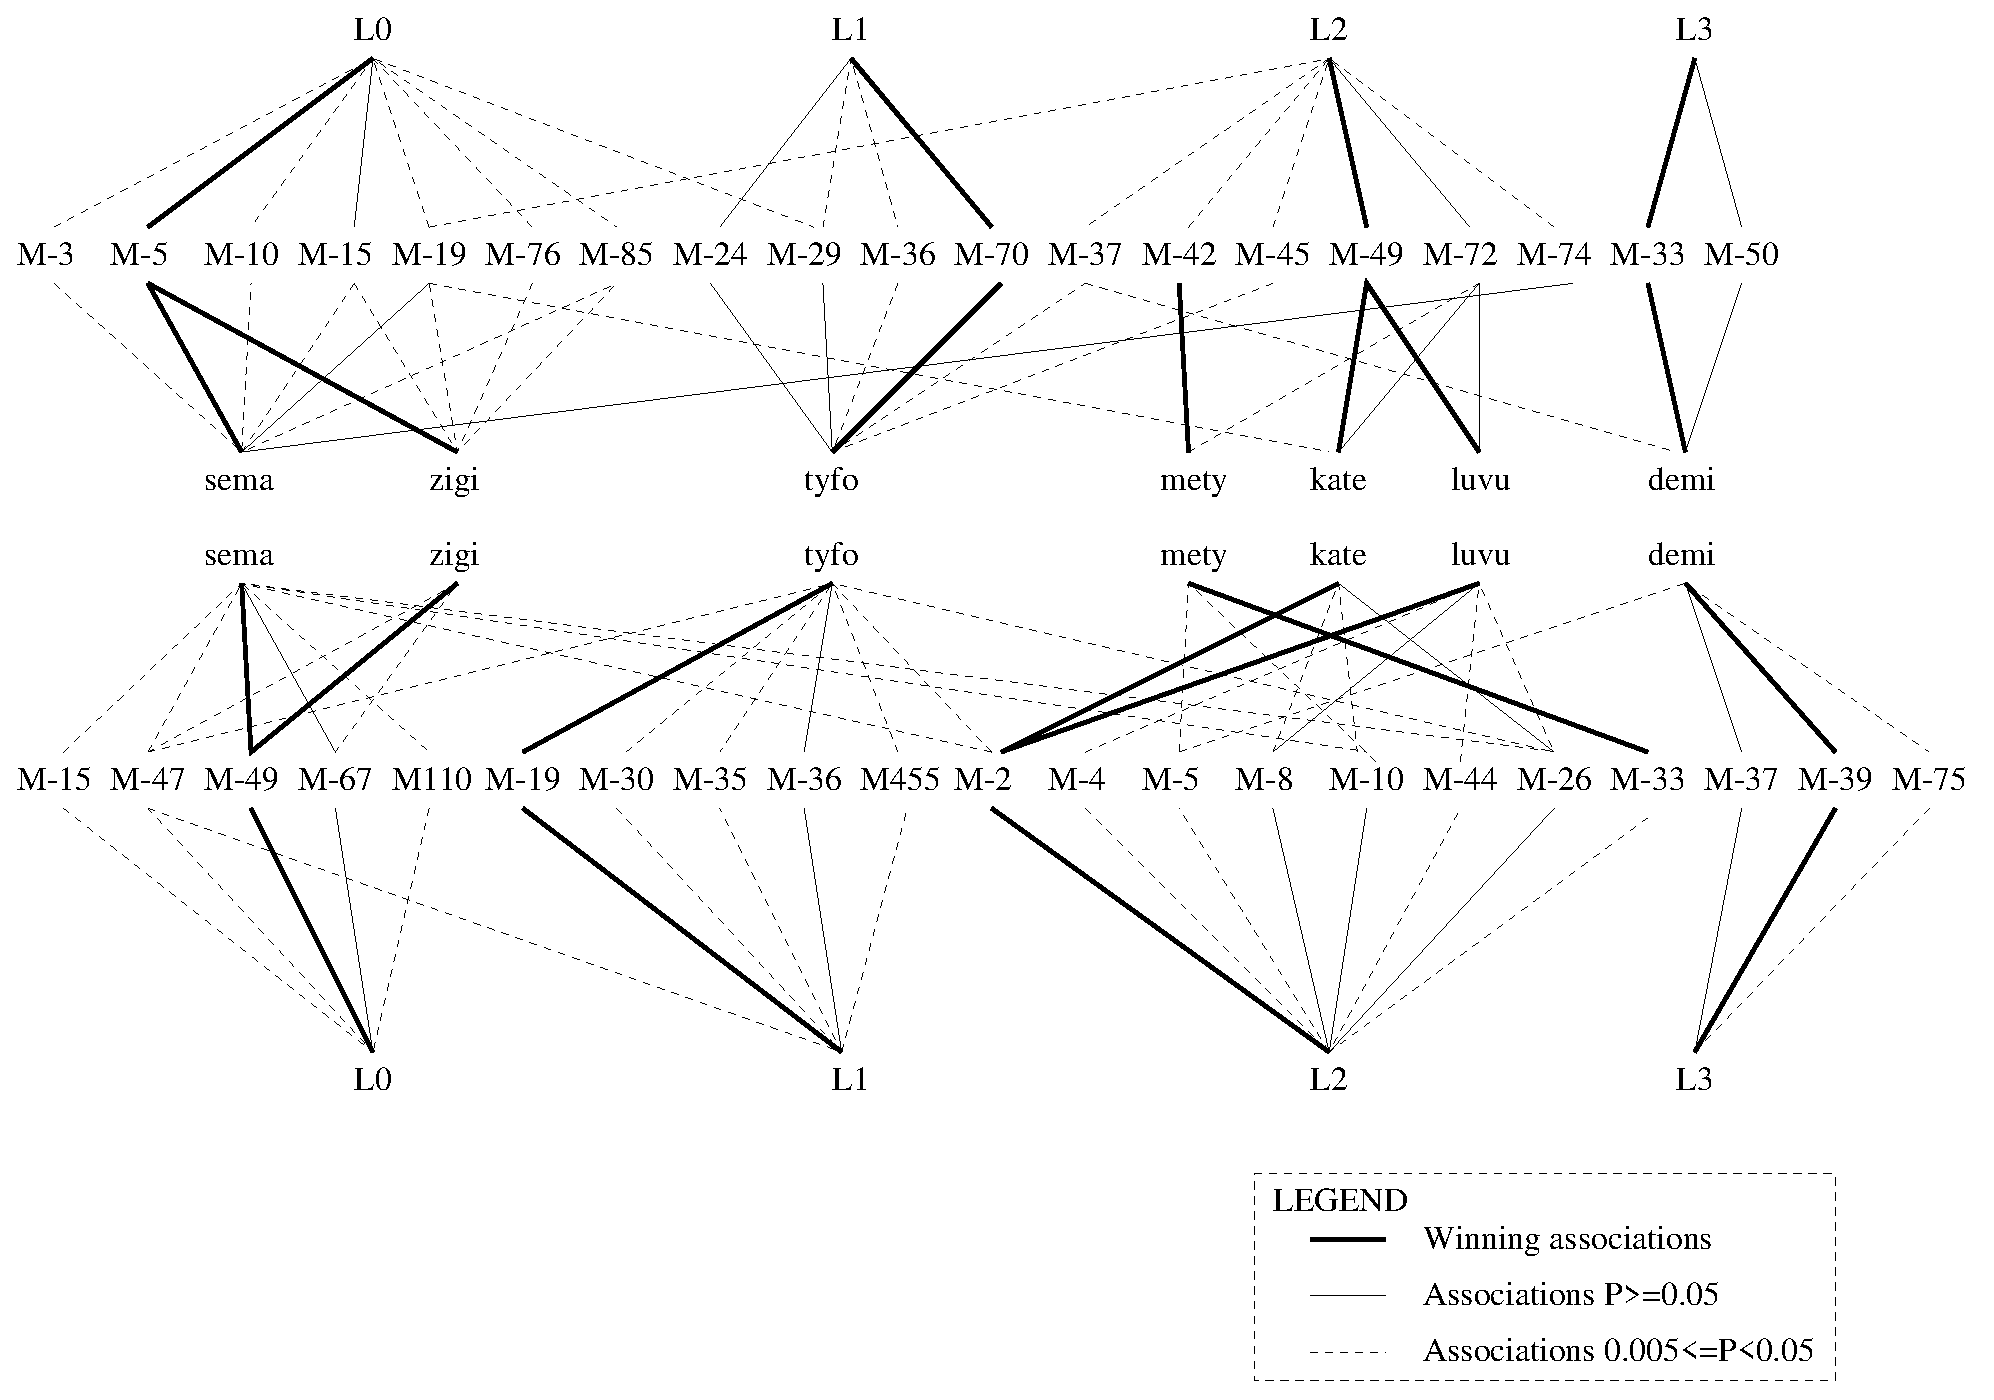
\includegraphics[width=12cm]{optimal/semiotic.eps}}
\caption{The semiotic landscape of the optimal experiment with $P_s=0.1$.}
\label{f:opt:semiotic}
\end{figure}

This orthogonality criterion is achieved for {\bf mety}, {\bf luvu} and possibly {\bf zigi}. The word-forms {\bf kate} and {\bf demi} have cross-connections, but these are relatively unimportant because they have low frequencies. More referential polysemy is found for {\bf sema} and {\bf tyfo}. As will be shown in the discussion, {\bf tyfo} gets well established to name L1 almost unambiguously. {\bf sema} however, provides some instability in the system. 

Comparing this landscape with that of the basic experiment (figure \ref{f:st:semiotic} at page \pageref{f:st:semiotic}), the system shows more orthogonality and there are less word-forms. L0 and L2 have synonymous connections, but these are not a big problem, since the different forms are most frequently used to name one referent, i.e. they show low polysemy.
\index{semiotic landscape|)}


One important result of experiment P.1 is that the number of word-forms the agents use {\em successfully} in the language is much lower than in P.4. The robots used 16 word-forms successfully at the end vs. 34 in P.4 (figure \ref{f:opt:words} (a), solid lower line). Furthermore, the number of word-forms does not grow after approximately 3,500 games, whereas the vocabulary size increases until the end when $P_s=0.4$. The number of word-forms that have been created by the robots is only slightly above the number of word-forms that have been successfully used. Apparently the robots tend to have more time to adopt word-forms correctly when $P_s=0.1$. \index{lexicon!growth|(}\index{ontology!growth|(}


\begin{figure}
\centering
\subfigure[word-forms]{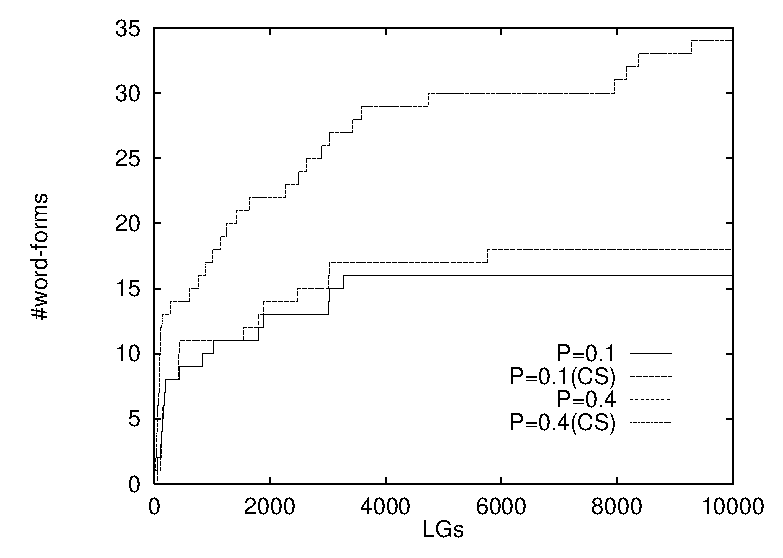
\includegraphics[width=5.5cm]{optimal/wordsopt.eps}}
\subfigure[concepts]{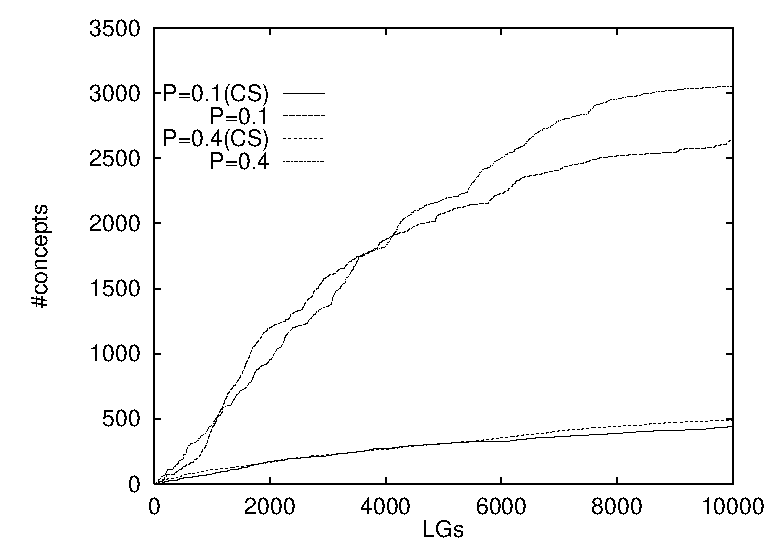
\includegraphics[width=5.5cm]{optimal/conceptsopt.eps}}
\caption{The vocabulary and ontological growth of experiments with P.1 and P.4. The growth is shown for successful usage (indicated with CS) and just those elements that are used. The concepts that are just used are those that have found to be distinctive.}
\label{f:opt:words}
\end{figure}

The one-to-many relations between form and meaning of both systems is high as can be derived from figure \ref{f:opt:words}. Figure \ref{f:opt:words} (b) shows the ontological growth of categories that are distinctive and of those that are successfully used in the communication (as indicated by (CS)) for creation probabilities $P_s=0.1$ and $P_s=0.4$. The total numbers of distinctive categories that the agents categorised are ranging from 2,600 for P.1 and 3,100 for P.4. The number of meanings (categories that are used in communication) they successfully use is around 500, which is substantially lower than the number of concepts that could be used. So, the number of successfully employed concepts is roughly $15 \times$ higher than the word-forms that are used when $P_s=0.4$ and it is $31 \times$ higher when $P_s=0.1$. It appears that in case when the creation probability is lower, the robots have more time to associate existing word-forms with meanings rather than to create new ones. This way the amount one-to-many relations between form and meaning increases as a possibly beneficial side effect. The cost of this is that there appears to be a higher level of polysemy. To see whether this is problematic, it is instructive to look at the various competition diagrams of experiment P.1. This is done in the discussion that follows.
\index{lexicon!growth|)}\index{ontology|growth|)}\index{lexicon|)}


\subsection{Discussion}

The results make clear that with the current settings and strategies, the robots construct a communication system that meets its limits. The communicative success is in the end nearly as high as the potential understandability. 

Both the discriminative success and distinctiveness are very close to 1, and the specificity is also close to 1. So, when a robot uses a symbol successfully, it almost always refers to the same referent. The polysemy is very low. The parsimony and consistency are somewhat lower. Hence, there are some one-to-many relations between referent and meaning and between referent and form in the system. The semiotic landscape already showed that most of the synonymy does not necessarily mean that the communication is difficult. Usually, the hearer can rather easily interpret any speaker's utterance. The landscape also shows that a one-to-many relationship between form and meaning does not necessarily mean polysemy. Moreover, it is beneficial, since it antagonises the one-to-many mapping of referent to meaning for a great deal. This is nicely illustrated by the following discussion of some competition diagrams that are taken from the same run as the semiotic landscape. The discussion also explains some of the dynamics of the language games.

\begin{figure}
\centering
\subfigure[RF-L1]{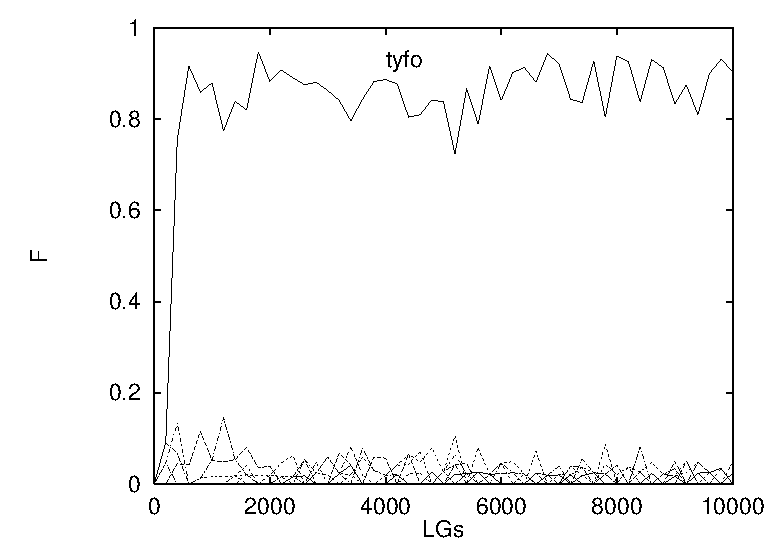
\includegraphics[width=5.5cm]{optimal/rf0-1p.eps}}
\subfigure[RF-L1-success]{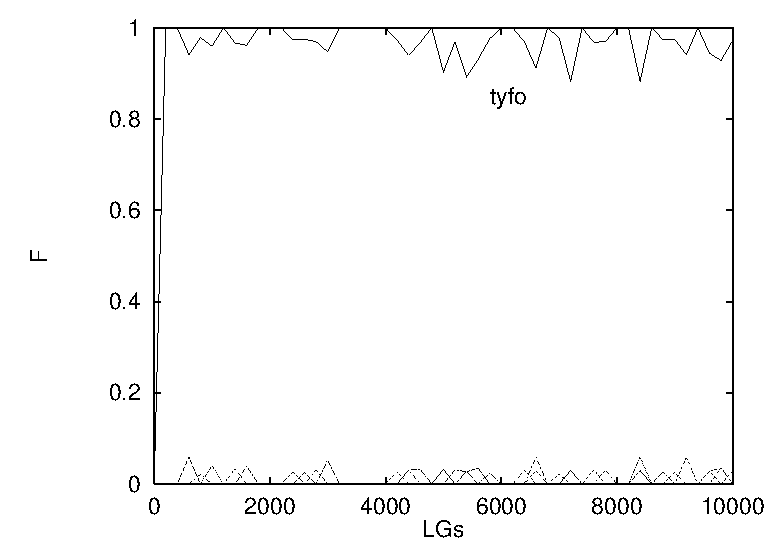
\includegraphics[width=5.5cm]{optimal/rf0-1cs.eps}}\\
\subfigure[RM-L1]{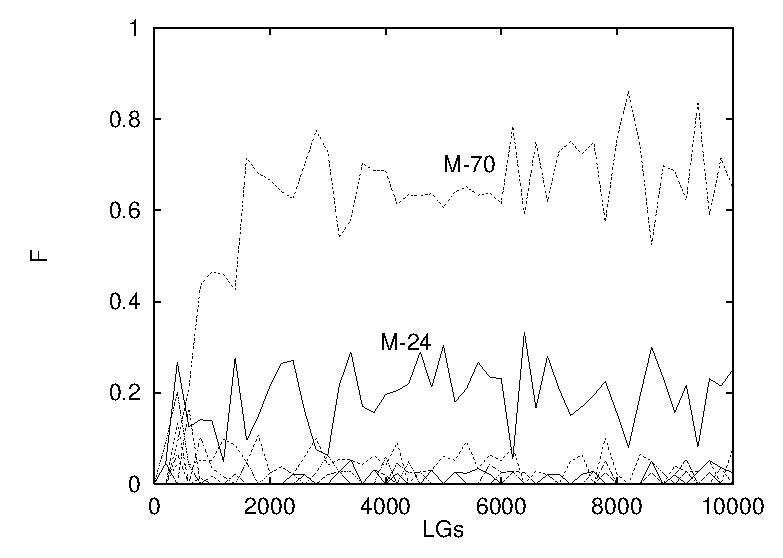
\includegraphics[width=5.5cm]{optimal/rc0-1p.eps}}
\subfigure[FM-tyfo]{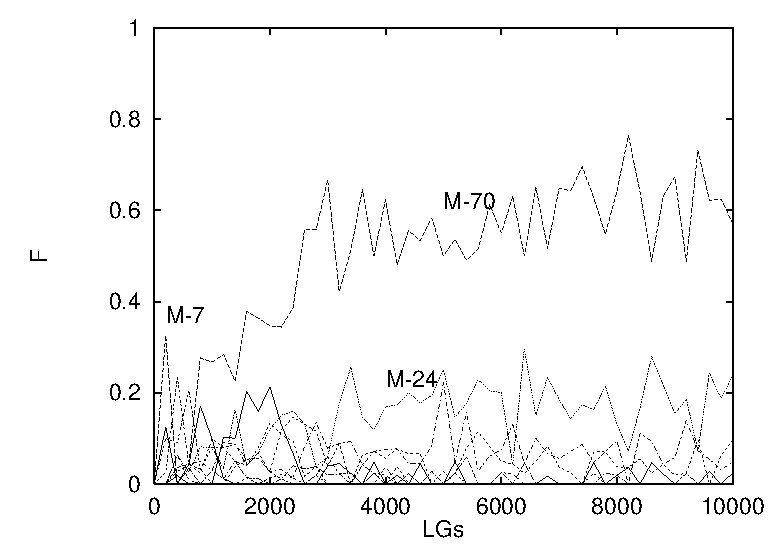
\includegraphics[width=5.5cm]{optimal/fc0-0p.eps}}\\
\subfigure[FR-tyfo]{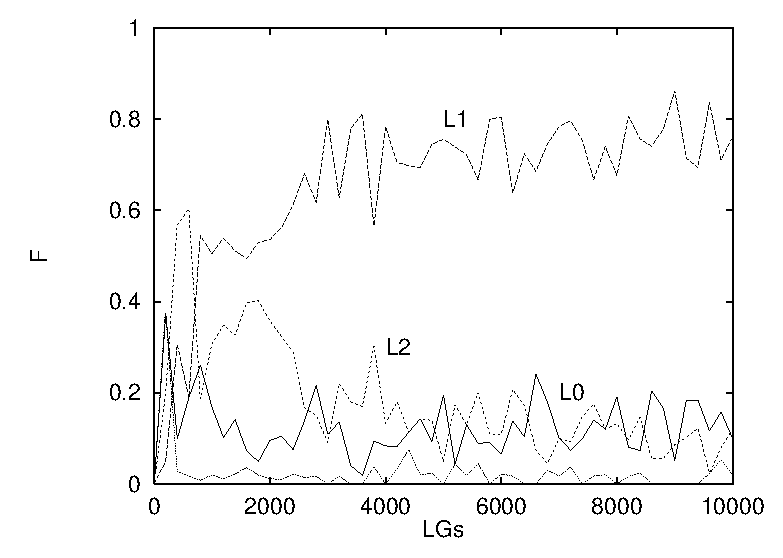
\includegraphics[width=5.5cm]{optimal/fr0-0p.eps}}
\subfigure[FR-tyfo-success]{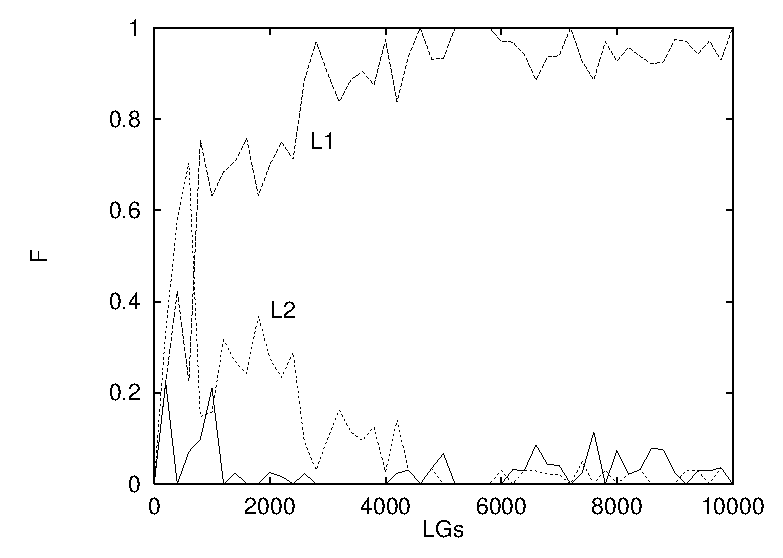
\includegraphics[width=5.5cm]{optimal/fr0-0cs.eps}}
\caption{Some competition diagrams of robot r0 in one run of experiment P.1. Figures (a) and (b) show referent-form competitions for L1, (a) show its use and (b) shows the successful use. Figure (c) shows the referent-meaning competition for L1 and (d) shows the form-meaning competition for {\bf tyfo}. Both figure (c) and (d) show the use. Figures (e) and (f) show the form-referent diagrams for {\bf tyfo}, where (e) shows its use, and (f) its effective use.\index{competition diagram}}
\label{f:opt:ggcomp1}
\end{figure}

\subsubsection{One-to-many Relations Between Form and Meaning}

Figure \ref{f:opt:ggcomp1} shows various competition diagrams of robot r0, relating to referent L1 in one of the runs of experiment P.1. Figures (a) and (b) show the referent-form competition. In figure (a) the co-occurrence frequencies of referent and form independent of their success are displayed. Figure (b) shows the successful co-occurrence of referent and form. Very infrequent occurrences are left out for clarity. Where figure (a) shows that form {\bf tyfo} clearly wins the competition, figure (b) shows that  in successful games, this form is nearly used uniquely\footnote{Note that this diagram is the same for robot r1, since it shows successful co-occurrences only. By definition of the success, they must be the same for both robots.}. Hence light source L1 has very little synonymy. \index{synonymy}

Although there is hardly any synonymy, there is substantial conceptual synonymy. This is nicely shown in the referent-meaning diagram for L1 (figure \ref{f:opt:ggcomp1} (c)). Two meanings are used rather frequently, M24 and M70. When looking at the form-meaning diagram for word-form {\bf tyfo} (figure (d)), a similar competition is observed. The frequent meanings that co-occur with {\bf tyfo} are M24 and M70. So, the lexical one-to-many relations between form and meaning antagonises out the negative side effect of the one-to-many relations between referent and meaning, yielding almost one-to-one relations between form and referent. So, there is little synonymy and polysemy. \index{polysemy}

That there is hardly any polysemy can be seen in figures \ref{f:opt:ggcomp1} (e) and (f). These figures plot the form-referent diagrams for used (e) and successfully used (f) co-occurrence frequencies. Although some polysemy can be observed, it is hardly present in successful games after, say, 4,000 language games.


\begin{table}
\centering
\begin{tabular}{cc}
\lsptoprule
M-5 & $(0.96,0.01,0.03,0.05)_1$\\%\hline
M-15 & $(0.96,0.60,0.03,0.05)_1$\\%\hline
M-19 & $(0.53,0.19,0.71,0.20)_0$\\%\hline
M-24 & $(0.38,0.99,0.03,0.05)_1$\\%\hline
M-33 & $(0.03,0.01,0.03,0.96)_1$\\%\hline
M-37 & $(0.03,0.01,1.00,0.96)_1$\\%\hline
M-49 & $(0.03,0.01,1.00,0.46)_1$\\%\hline
M-50 & $(0.03,0.01,0.28,0.96)_1$\\%\hline
M-70 & $(0.03,0.99,0.03,0.05)_1$\\%\hline
M-72 & $(0.03,0.01,1.00,0.05)_1$\\%\hline
\lspbottomrule
\end{tabular}
\caption{The legend of some meanings of robot r0 in the optimal guessing game as represented by their prototypes. It should be clear that the meanings mostly bare the invariant\index{invariance} property that the sensory channels have values (near) 1 corresponding to the referents they are used for\index{correspondence} which has values in the middle. This meaning acts at feature space ${\mathcal F}_0$, which can only be distinctive if there is only 1 referent in the context of a language game. This meaning is mainly used to categorise L0, although not very frequently. The semiotic landscape (figure \ref{f:opt:semiotic} shows that M19 (in the upper half) is also used to categorise L2. Another interesting meaning is M-37, which has high values in dimensions WL2 and WL3. It has been used most frequently to categorise L2 in the beginning of the experiments. Later it has been used less frequently. M-49 shows that the sensory channel WL3 adjacent to the corresponding sensory channel WL2 reads relatively high values when the robot detects L2. This can be inferred from the fact that both dimensions WL1 and WL3 have high values. That this does not happen all the time is shown with M-72, which has low values in each dimension that does not correspond with L2.}
\label{t:opt:legend}
\end{table}

Table \ref{t:opt:legend} shows the legend of some of the meanings that are discussed. Note that most meanings are uniquely used to stand for a particular referent. So, there are mostly one-to-one relations between meaning and referent, which drives the distinctiveness near 1, cf. figure \ref{f:opt:mr}.

\begin{figure}[t]
\centering
\subfigure[MR-M70]{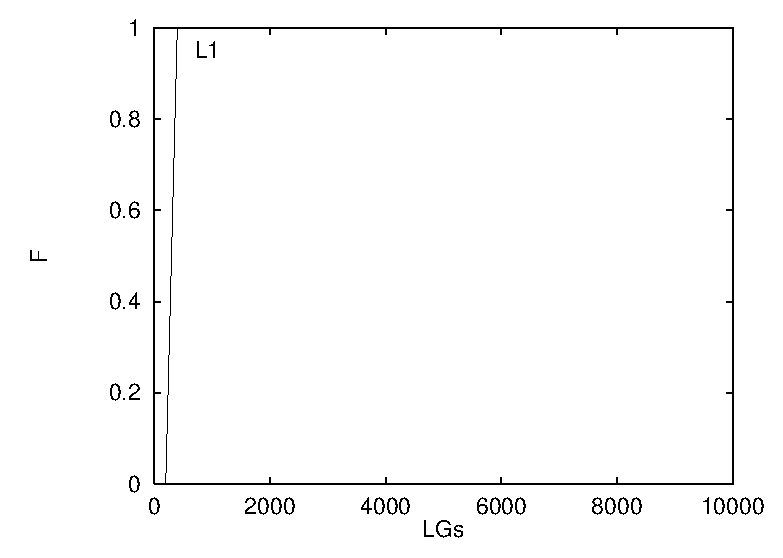
\includegraphics[width=5.5cm]{optimal/rc0-70p.eps}}
\subfigure[MR-M72]{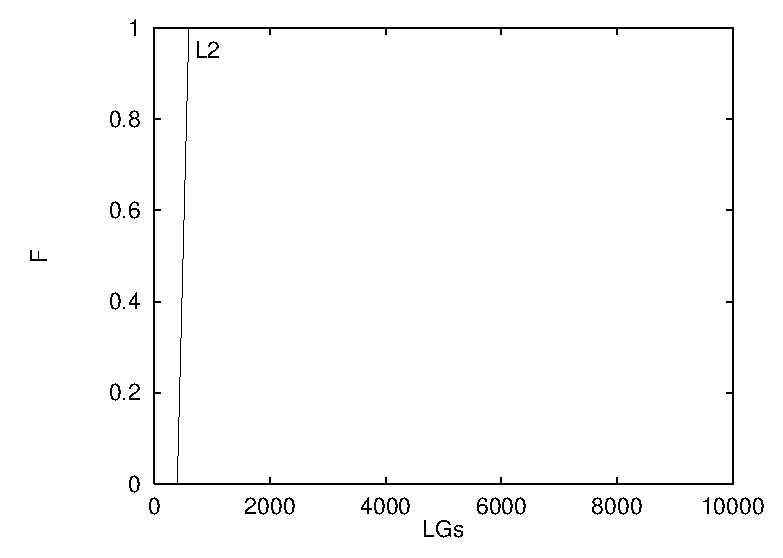
\includegraphics[width=5.5cm]{optimal/rc0-72p.eps}}
\caption{Meaning-referent competition of r0 for meanings M70 and M72.}
\label{f:opt:mr}
\end{figure}

\subsubsection{Polysemy and Lexical Dynamics}\index{polysemy|(}

\begin{figure}
\centering
\subfigure[RF-L2]{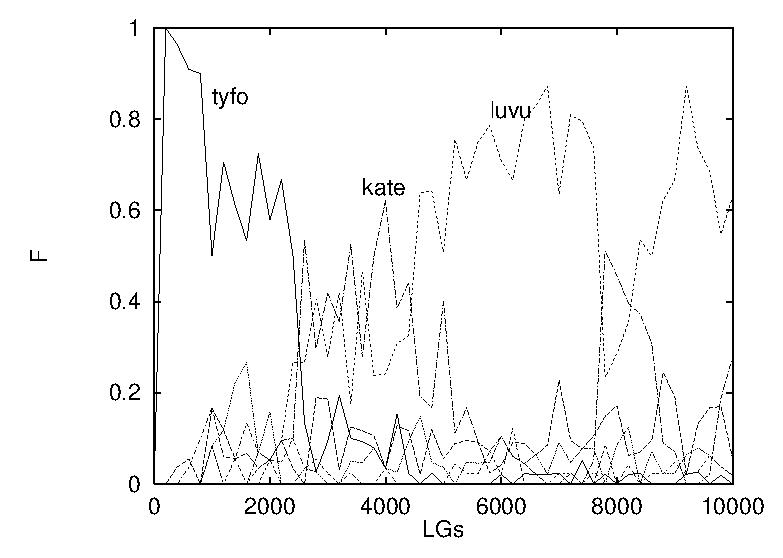
\includegraphics[width=5.5cm]{optimal/rf0-2cs.eps}}
\subfigure[RM-L2]{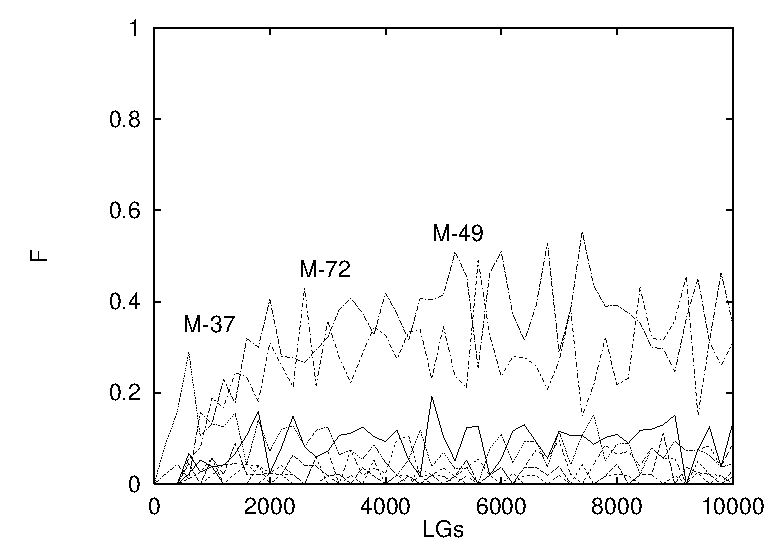
\includegraphics[width=5.5cm]{optimal/rc0-2p.eps}}\\
\subfigure[MF-M49]{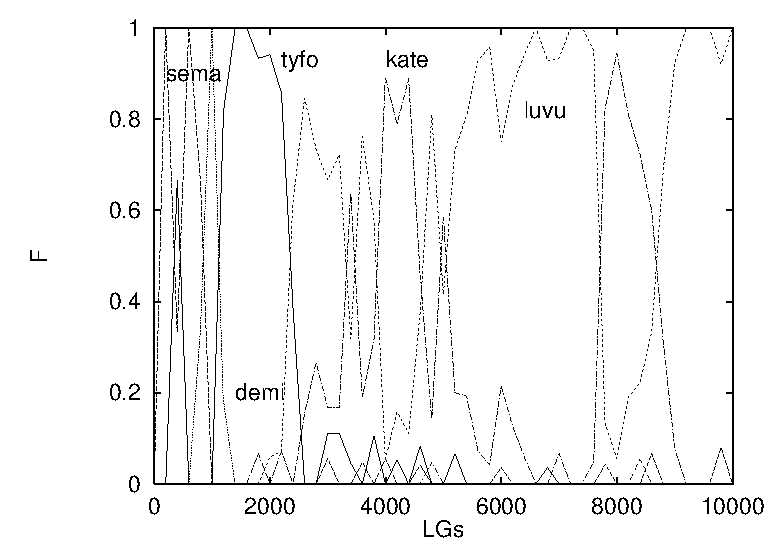
\includegraphics[width=5.5cm]{optimal/cf0-49p.eps}}
\subfigure[MF-M72]{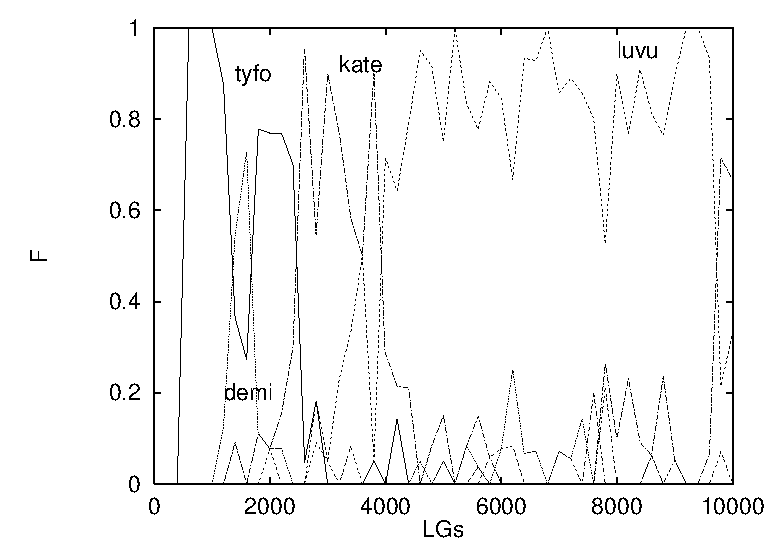
\includegraphics[width=5.5cm]{optimal/cf0-72p.eps}}\\
\subfigure[FM-luvu]{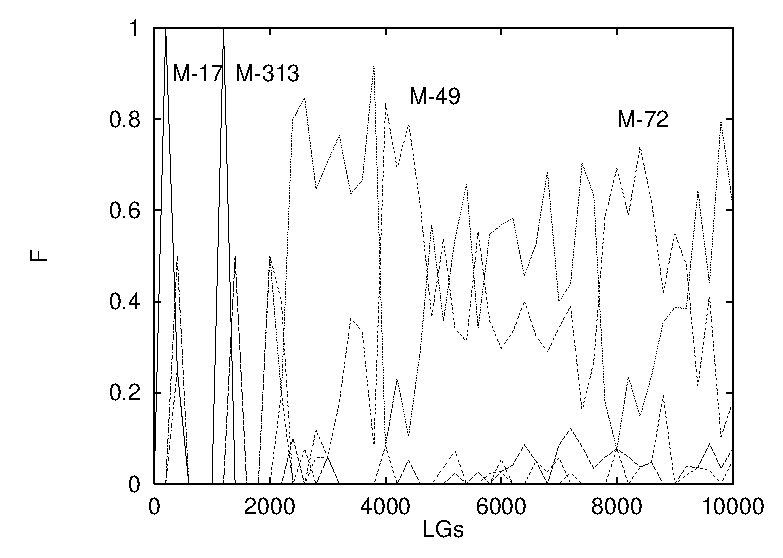
\includegraphics[width=5.5cm]{optimal/fc0-4p.eps}}
\subfigure[FM-kate]{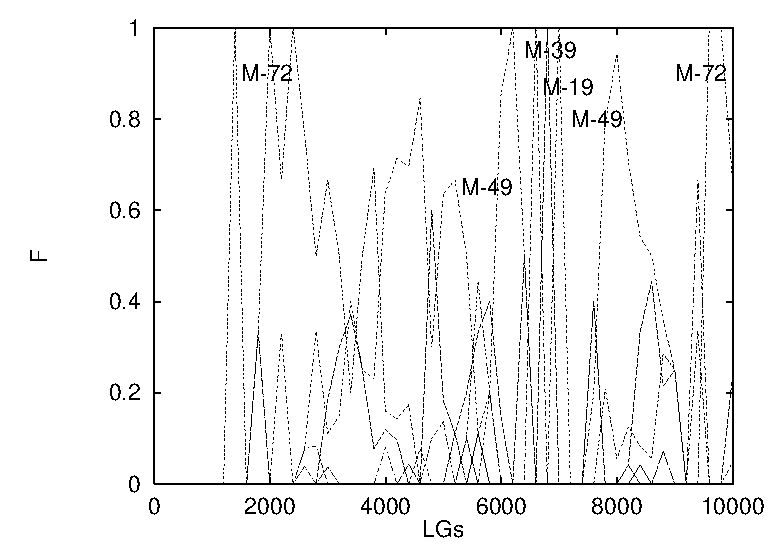
\includegraphics[width=5.5cm]{optimal/fc0-8p.eps}}
\end{figure}
\begin{figure}
\centering
\subfigure[FR-luvu]{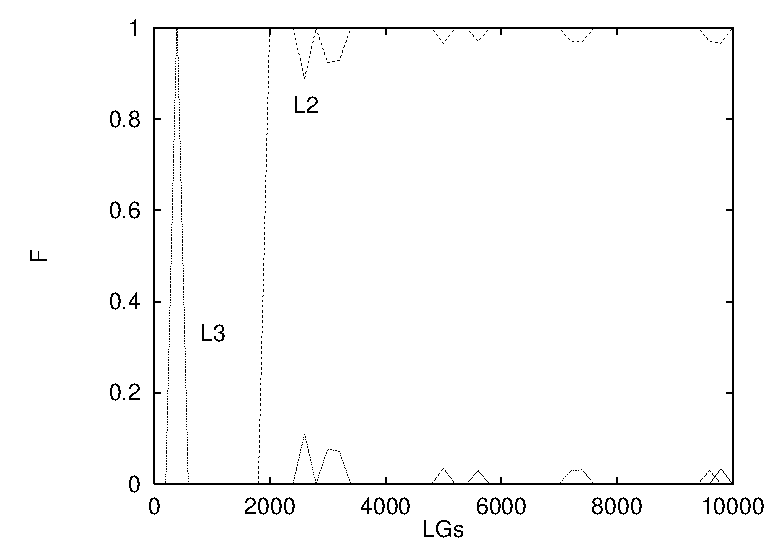
\includegraphics[width=5.5cm]{optimal/fr0-4cs.eps}}
\subfigure[FR-kate]{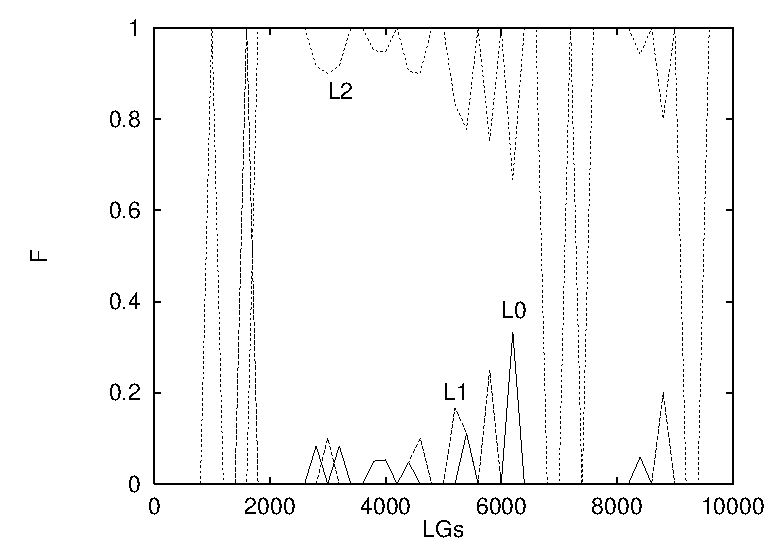
\includegraphics[width=5.5cm]{optimal/fr0-8cs.eps}}
\caption{Various competition diagrams of r0 concerning light source L2. The referent-form (a) and form-referent diagrams (g) and (h) display competitions of successful occurrences. All other diagrams show competitions of used occurrences.}
\label{f:opt:ggcomp2}
\end{figure}

That relations and competition between referent, meaning and form are not always as nice as in the case above is shown in figure \ref{f:opt:ggcomp2}. The competition is taken from the same run as the semiotic landscape and the previous example, so $P_s=0.1$.

Figure \ref{f:opt:ggcomp2} (a) shows the referent-form diagram of successful co-occurrences of referent L2 with some forms. After an initial period in which {\bf tyfo} is used, the diagram is dominated by a competition between {\bf luvu} and {\bf kate}. It appears as if {\bf luvu} is the most dominant of the two. To investigate this competition in more detail, one should look at the referent-meaning diagram (figure \ref{f:opt:ggcomp2} (b)).

The referent-meaning diagram shows that there appear to be two meanings which are used more or less equally frequent: M49 and M72. There are more meanings that compete at the bottom of the graph. Apparently there is a strong one-to-many relation between referent and meaning. 

Figures (c) and (d) show the MF diagrams of the two dominant meanings. It should be clear that a weighted superposition of the two diagrams resemble the referent-form diagram very much. Hence these diagrams also show the dynamic competition between {\bf luvu} and {\bf kate}. So, the synonymous referent-form competition cannot directly be explained by the fact that L2 is categorised by two meanings. These meanings themselves show similar mappings between referent and meaning. This is not so odd, since light source L1 (figure \ref{f:opt:ggcomp1}) was not named with two forms, whereas it is related with two meanings.

The apparently unstable competition returns in the form-meaning diagrams of the two relevant forms (figures \ref{f:opt:ggcomp2} (e) and (f)). {\bf luvu}, which appears to be the most dominant form for L2, evolves in a competition between M49 and M72. The competition for {\bf kate} appears to be more chaotic. This is probably due to the fact that {\bf kate} is used infrequent in the period where it shows most chaos (between game 6,000 and 7,000).

It is difficult to tell exactly what factors cause the dynamic competition. There are many factors that can influence the dynamics of language games that it seems impossible to explain what happened. The most important factors are the adaptation of association scores, its lateral inhibition, the one-to-many relation between referent and meaning, the different ontologies and lexicons of the robots, the different contexts and situations, language game failures and possibly many more. The observed dynamics are probably caused by an interaction between these factors.


So, although it is not completely understood, here follows a possible explanation. In the periods where {\bf kate} is more (or even most) dominant in the competition, M49 appears to be the most dominant meaning in the form-meaning competition for {\bf kate} and least dominant for {\bf luvu}. Check the periods around games 4,000 and 8,000. This is also observable in the MF competition for M49.

If one looks at the meaning-form competition for M72, {\bf kate} is the dominant form in the period between 3,000 and 4,000, just before it becomes dominant for M49. In this period, the other robot (r1) must have acquired {\bf kate} and uses it also to name L2. Through the linguistic interactions it is not unlikely that our robot (r0) starts to use {\bf kate} also successfully for M49. The association scores are laterally inhibited, so when {\bf kate} is successfully used to name M49, this association is strengthened, but the associations between {\bf kate} and M72, and {\bf luvu} and M49 are inhibited.

If such dynamics continues, there will be a break point where there is a trade off between the dominant associations. At that point, {\bf kate} may become dominant M49, and {\bf luvu} becomes dominant for M72. This dominance is very stable until the end of the run where {\bf kate} starts to win again. A short while after {\bf luvu} became dominant for M72, it also started to win the competition for M49.

It seems as the dominance for one meaning is taken over by the dominance for the other meaning. This take over is antagonised with the take over of another form for the first meaning. This in turn can feed the competition similarly; thus a vicious circle emerges.


To finish the discussion, look at figures (g) and (h). These figures show the form-referent diagrams of successfully used occurrences of {\bf luvu} (g) and {\bf kate} (h). Clearly these forms are specifically used to name L2. So, there is huge competition showing one-to-many relations between referent and meaning, meaning and form, and form and meaning. However, there is little polysemy. Note by the way that {\bf kate} is not used successfully at all around game 7,000.

\index{polysemy|)}

\section{The Observational Game}\label{s:opt:oli}
\index{observational game|(}
\index{joint attention|(}

\subsection{The Experiment}

The final experiment that will be reported is the experiment in which there is joint attention, but no feedback available to the agents. Hence the robots play observational games. The experiment takes the same improved parameters as the guessing game, see table \ref{t:opt:oli}. However, it only investigates form creation probability $P_s=0.4$. Note that the robots have no extra word-form adoption, since for this mechanism the robots have to know whether they mismatched in referent. For this they would need feedback, which the observational game lacks. Besides the robots know already what the topic is, so they will not be able to find a mismatch in referent.

\begin{table}[t]
\centering
\begin{tabular}{cc}
\lsptoprule
Type of change & Value\\\midrule
data-set & new gearing\\%\hline
$P_s$ & 0.4\\%\hline
$\eta$ & 0.9\\%\hline
Adoption scheme & N.A.\\%\hline
\lspbottomrule
\end{tabular}
\caption{The set-up of the optimal observational game. }
\label{t:opt:oli}
\end{table}

\subsection{The Results}

\begin{figure}
\centering
\subfigure[CS]{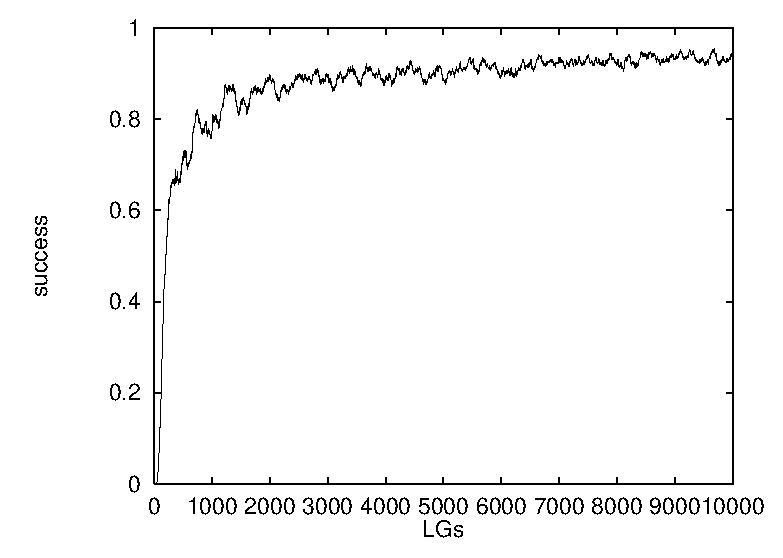
\includegraphics[width=5.5cm]{optimal/csoli.eps}}
\subfigure[DS]{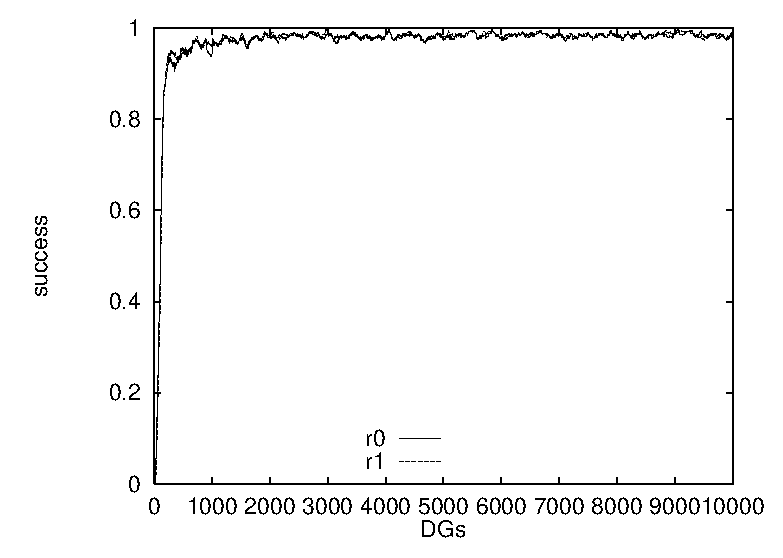
\includegraphics[width=5.5cm]{optimal/dsoli.eps}}
\subfigure[S]{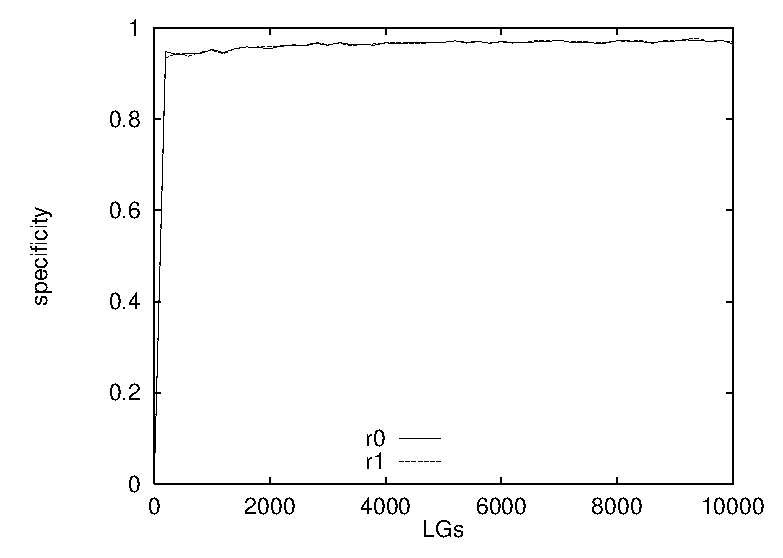
\includegraphics[width=5.5cm]{optimal/soli.eps}}
\subfigure[D]{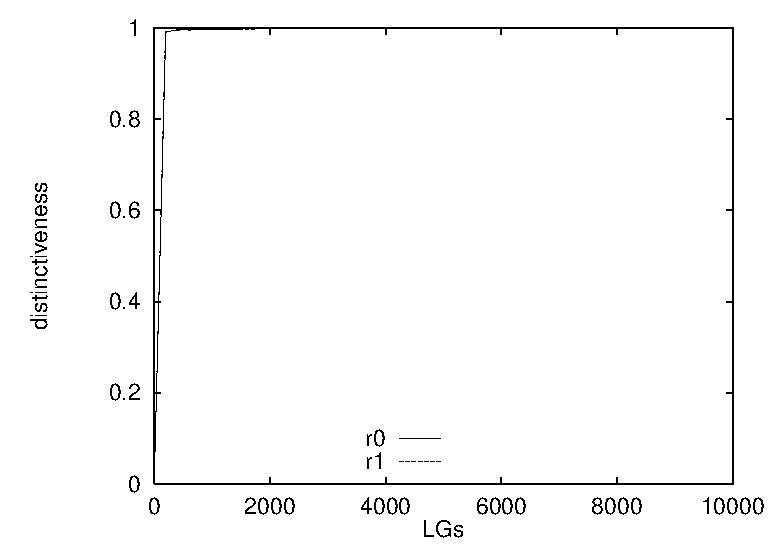
\includegraphics[width=5.5cm]{optimal/doli.eps}}
\subfigure[C]{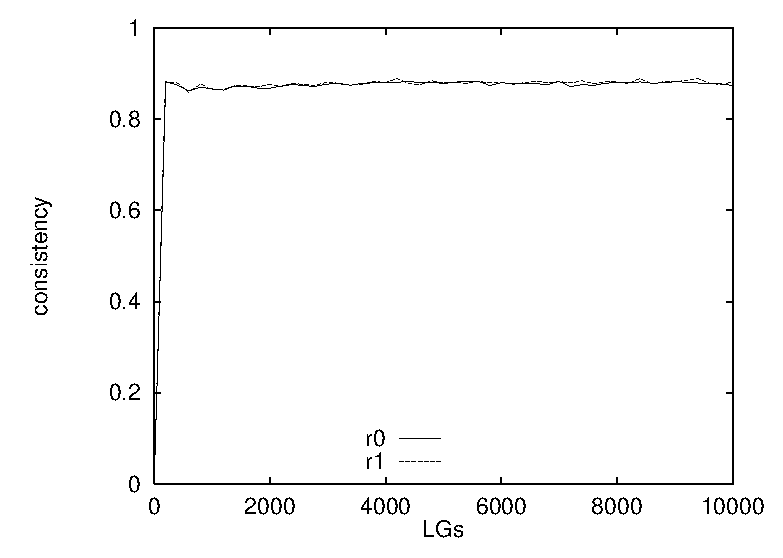
\includegraphics[width=5.5cm]{optimal/coli.eps}}
\subfigure[P]{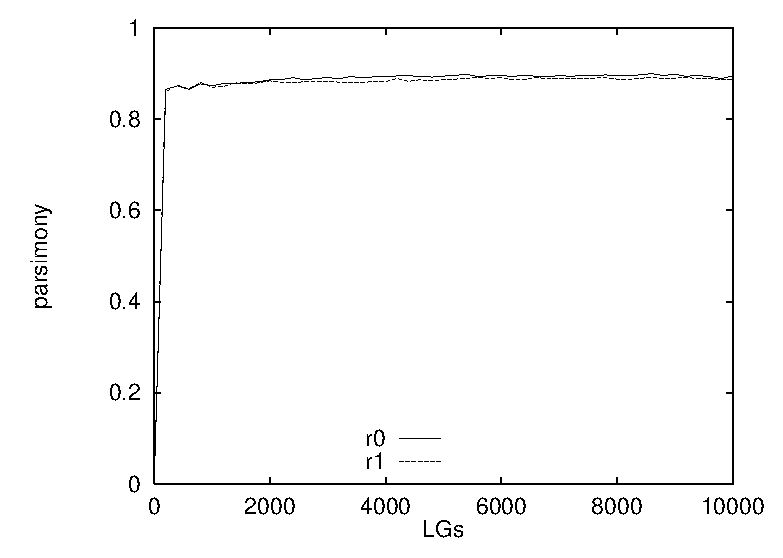
\includegraphics[width=5.5cm]{optimal/poli.eps}}
\end{figure}
\begin{figure}
\centering
\subfigure[AS]{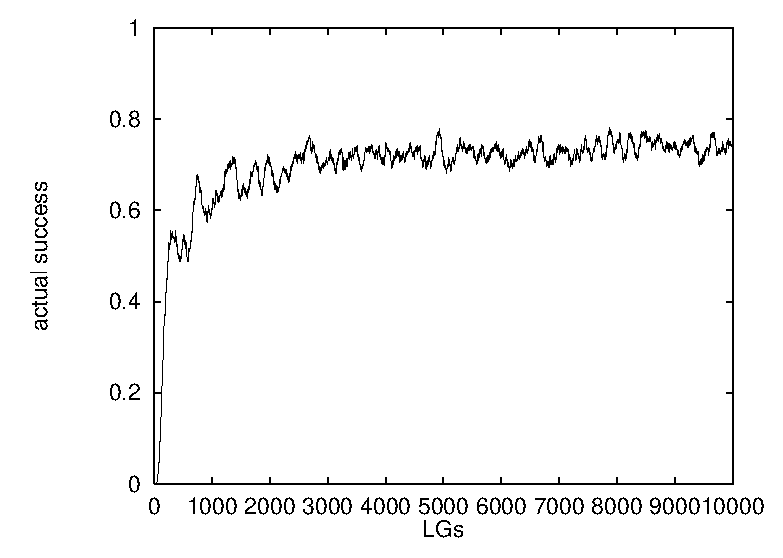
\includegraphics[width=5.5cm]{optimal/asoli.eps}}
\caption{The results of the optimal observational game.}
\label{f:opt:plotoli}
\end{figure}

\begin{table}
\centering
\begin{tabular}{lc}
\lsptoprule
Score & Avg \\\midrule
CS & 0.879$\pm$0.005\\%\hline
AS & 0.698$\pm$0.003\\%\hline
DS0 & 0.973$\pm$0.000\\%\hline
DS1 & 0.974$\pm$0.000\\%\hline
D0 & 0.979$\pm$0.000 \\%\hline
D1 & 0.979$\pm$0.000 \\%\hline
P0 & 0.873$\pm$0.001\\%\hline
P1 & 0.867$\pm$0.001\\%\hline
S0 & 0.946$\pm$0.004\\%\hline
S1 & 0.946$\pm$0.005\\%\hline
C0 & 0.860$\pm$0.006\\%\hline
C1 & 0.862$\pm$0.006\\%\hline
\lspbottomrule
\end{tabular}
\caption{The averaged results of the optimal observational game experiment.}
\label{t:opt:oli1}
\end{table}

The results of this experiment are shown in figure \ref{f:opt:plotoli} and table \ref{t:opt:oli1}. As the figure and table make clear, the global measures have similar results as the guessing game. Except the actual success is about 6 \% higher than the communicative success of this experiment ($p=0.0000$). Note that the actual success of the guessing game is the same as its communicative success, because the feedback of the guessing game is provided by the correspondence criterion. 

\subsection{Discussion}

Apparently the observation game yield better results than the guessing game. It seems that the robots are better at developing a lexicon when they know what the topic in advance rather than when they need feedback to guide their success. If the guessing game would not be able to construct a similar system is not proven. However, it would certainly take longer (compare figures  \ref{f:opt:ggplots} with\ref{f:opt:plotoli}).

Does the observational games yield a similar evolution of word-form and meaning? To see this, one can investigate the various competition diagrams. The referent-form competition diagrams (figure \ref{f:opt:rfoli}) shows the successful co-occurrences of one of the runs of this experiment. 

\begin{figure}[t]
\centering
\subfigure[L0]{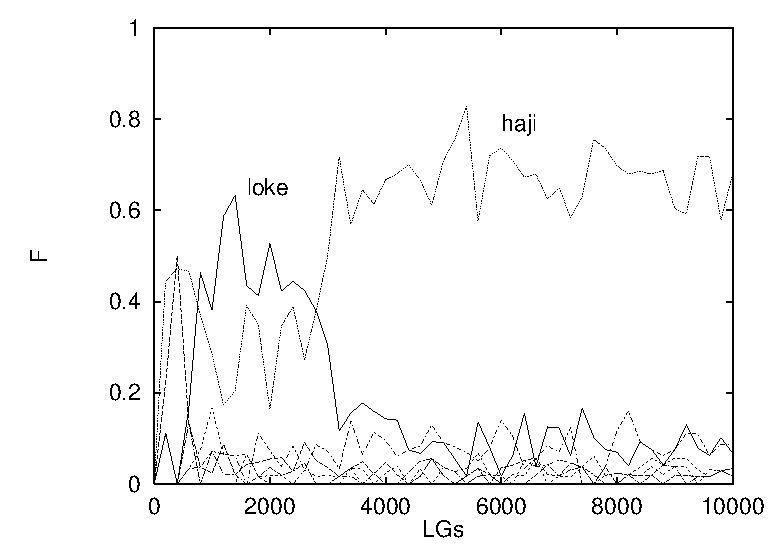
\includegraphics[width=5.5cm]{optimal/rf0-0oli.eps}}
\subfigure[L1]{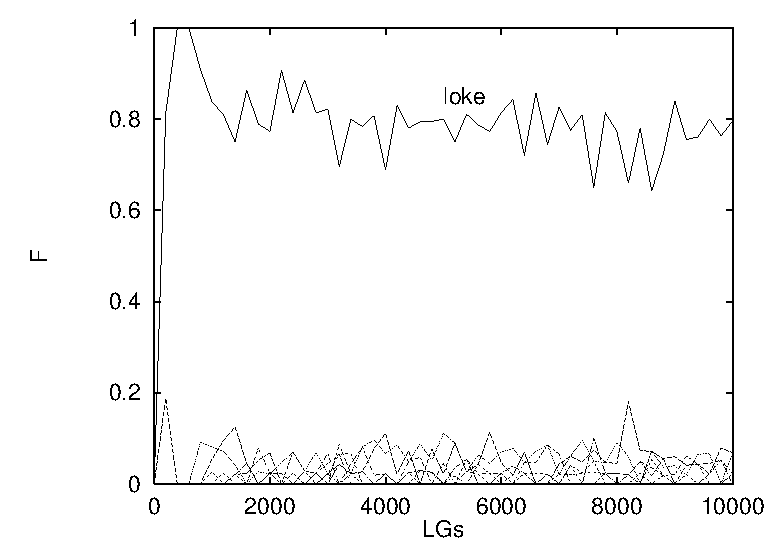
\includegraphics[width=5.5cm]{optimal/rf0-1oli.eps}}
\subfigure[L2]{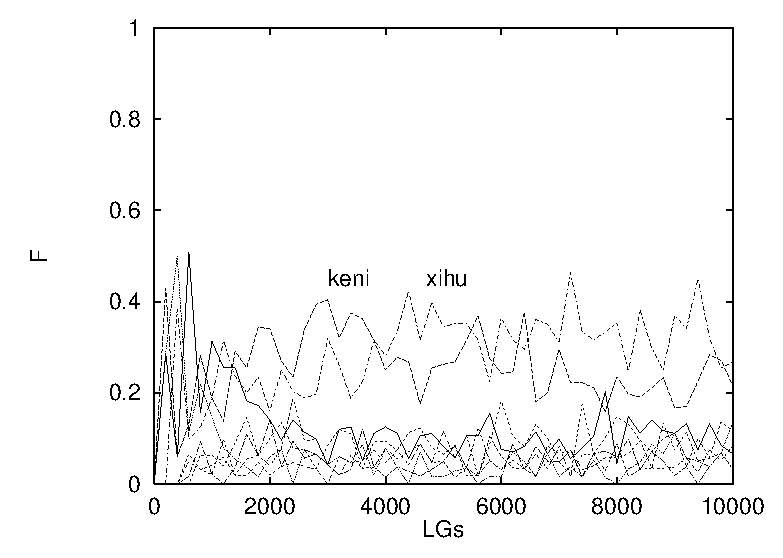
\includegraphics[width=5.5cm]{optimal/rf0-2oli.eps}}
\subfigure[L3]{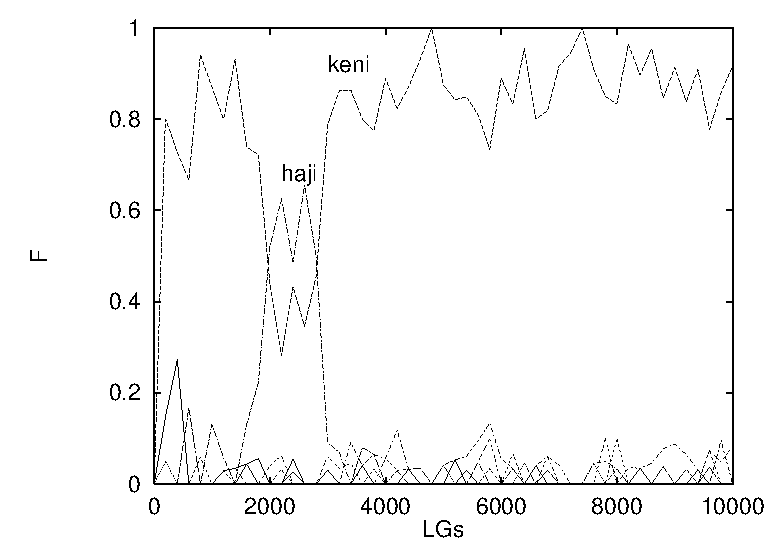
\includegraphics[width=5.5cm]{optimal/rf0-3oli.eps}}
\caption{Referent-form diagrams of the observational language game.}
\label{f:opt:rfoli}
\end{figure}

For three out of four referents there are clear winning word-forms, although light sources L0 and L3 both show a short period where another word-form takes over. L2 does not show a clear winning word-form. Two word-forms are used with almost the same frequency. One of these word-forms {\bf keni} is used to name both L2 and L3. Hence there is apparently some polysemy, see also figure \ref{f:opt:froli}. This has not been observed at this level in the guessing game.

\begin{figure}[t]
\centering
\subfigure[haji]{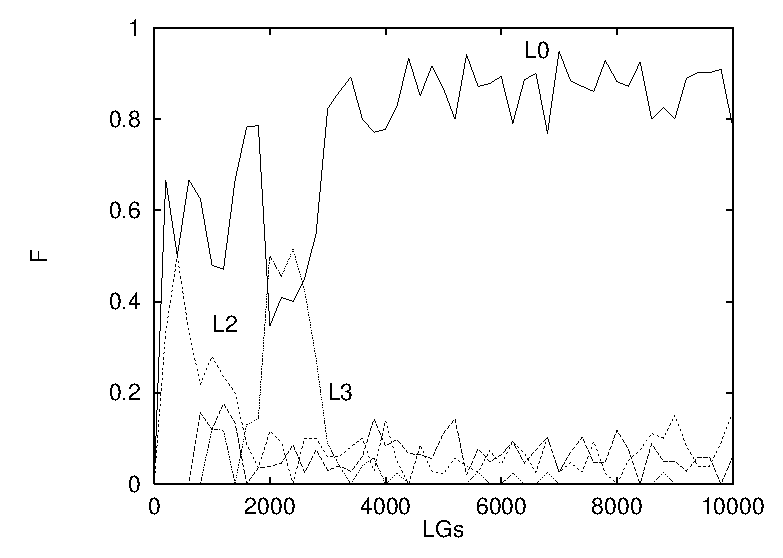
\includegraphics[width=5.5cm]{optimal/fr0-8oli.eps}}
\subfigure[loke]{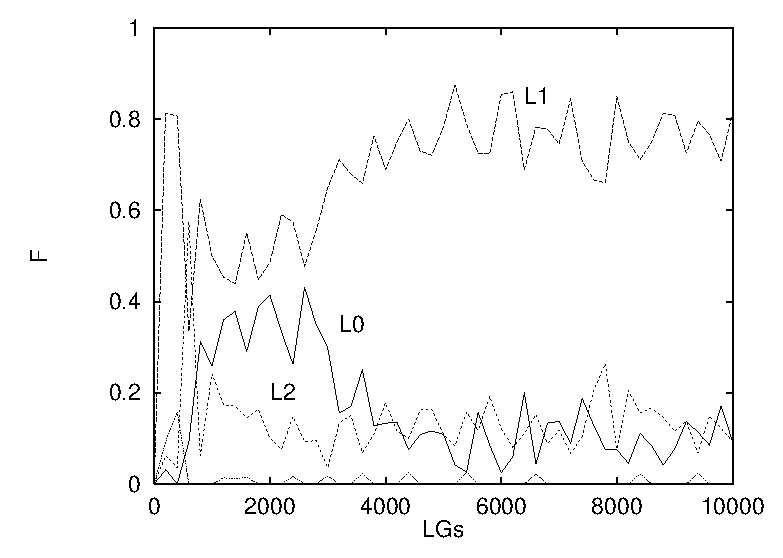
\includegraphics[width=5.5cm]{optimal/fr0-1oli.eps}}
\subfigure[xihu]{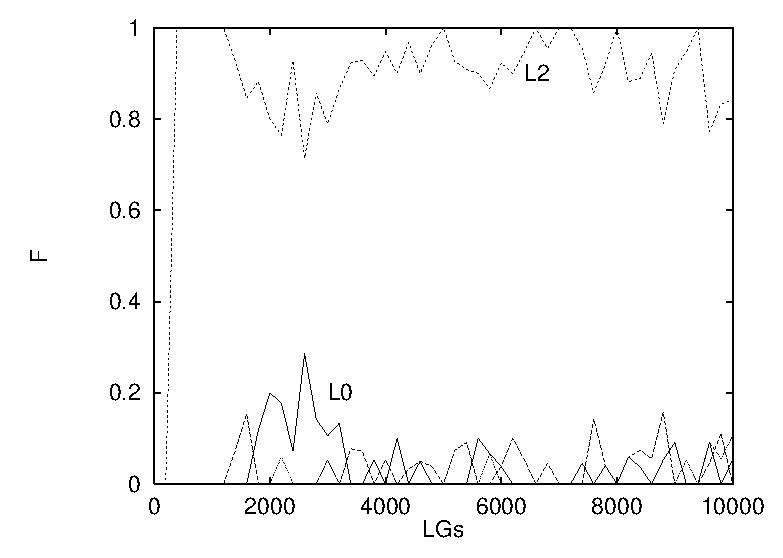
\includegraphics[width=5.5cm]{optimal/fr0-12oli.eps}}
\subfigure[keni]{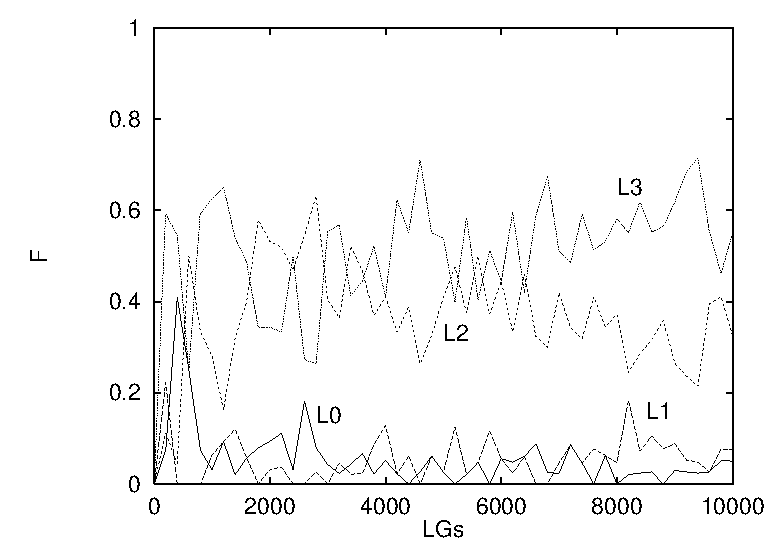
\includegraphics[width=5.5cm]{optimal/fr0-2oli.eps}}
\caption{Form-referent diagrams of the observational games.}
\label{f:opt:froli}
\end{figure}


Figure \ref{f:opt:froli} shows that there is some polysemy, especially for {\bf keni}.\index{polysemy} So, it would be interesting how the competition around {\bf keni} evolves. It is good to begin with some referent-meaning diagrams of both robots for light sources L2 and L3 (figure \ref{f:opt:rcoli}). From these figures it is clear that for L2 there is a high level of one-to-many mappings between referent and meaning, whereas L3 does not show this very much. Striking is that it is almost equally strong for both robots. Apparently, the synonymy in the lexicon reflects itself on these one-to-many relations between referent and meaning for both robots. It is not unlikely that one of the robots took over these one-to-many relations in its effort to disambiguate the synonymy initiated by the other. \index{synonymy}

For robot r0 there are basically three meanings that compete for light sources L2 and L3. The meaning-form competitions of these meanings are shown in figures \ref{f:opt:cfoli} (a) to (c). Meaning M-12, which is used to categorise L3 almost unambiguously, has very little synonymy and {\bf keni} clearly wins the competition. This is not very surprising, since L3 is both categorised  parsimonious and named consistent. The two meanings of L2 (M-28 and M-36) reveal more one-to-many relations between meaning and form. For M-12, {\bf keni} is most frequently used and for M-36 this is {\bf xihu}. In both cases the other name is also competing for these meanings, i.e. {\bf xihu} is also competing for M-12 and {\bf keni} for M-36. This competition, however is at a low level. The polysemy of {\bf keni} is also found back at the lexical level (i.e. in the one-to-many relations between form and meaning), cf. figure \ref{f:opt:cfoli} (d). \index{polysemy}

\begin{figure}[t]
\centering
\subfigure[L2-r0]{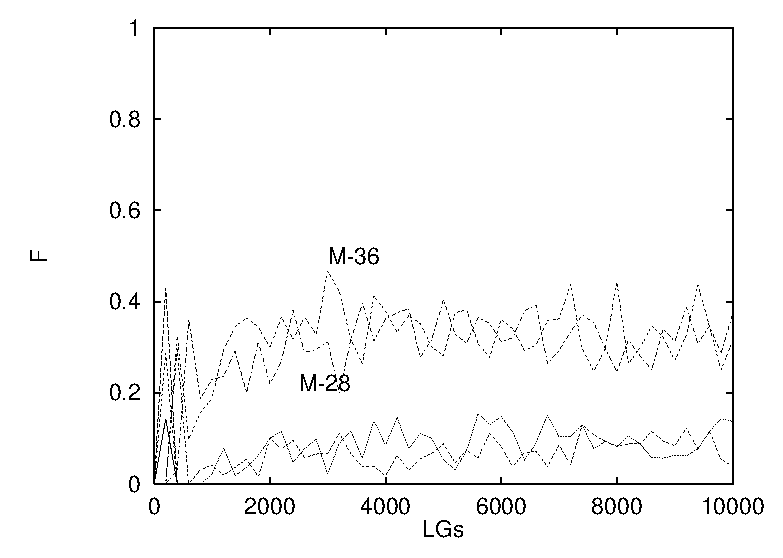
\includegraphics[width=5.5cm]{optimal/rc0-2oli.eps}}
\subfigure[L3-r0]{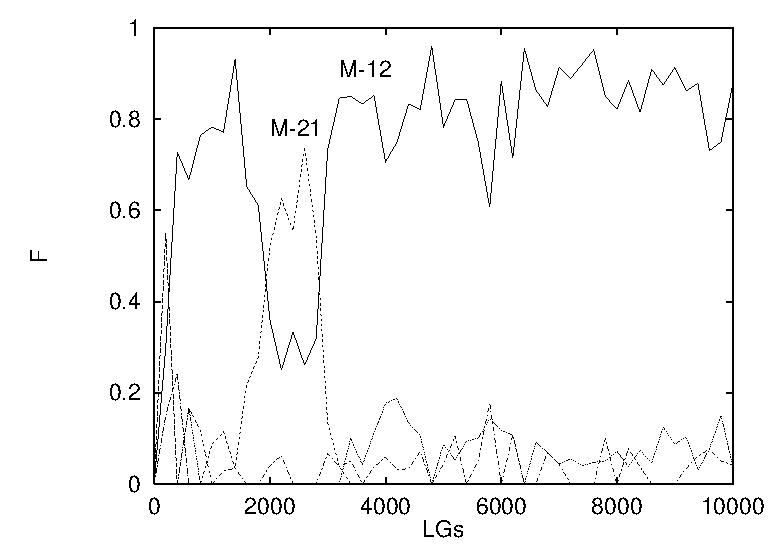
\includegraphics[width=5.5cm]{optimal/rc0-3oli.eps}}
\subfigure[L2-r1]{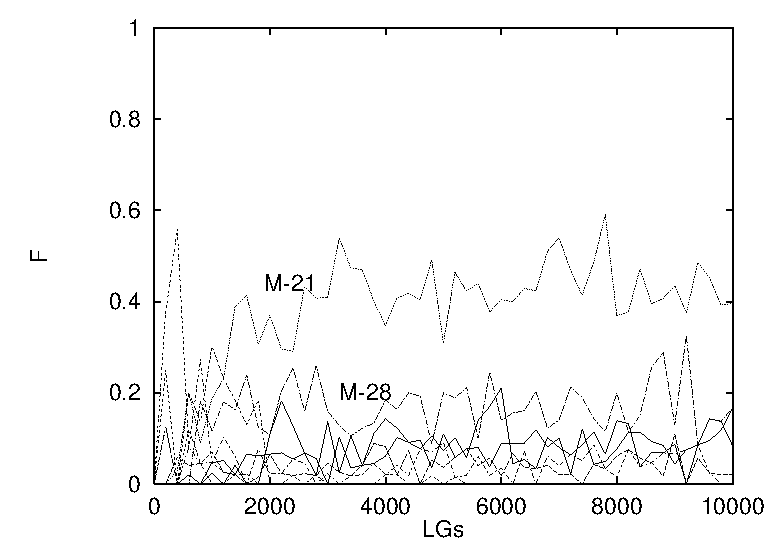
\includegraphics[width=5.5cm]{optimal/rc1-2oli.eps}}
\subfigure[L3-r1]{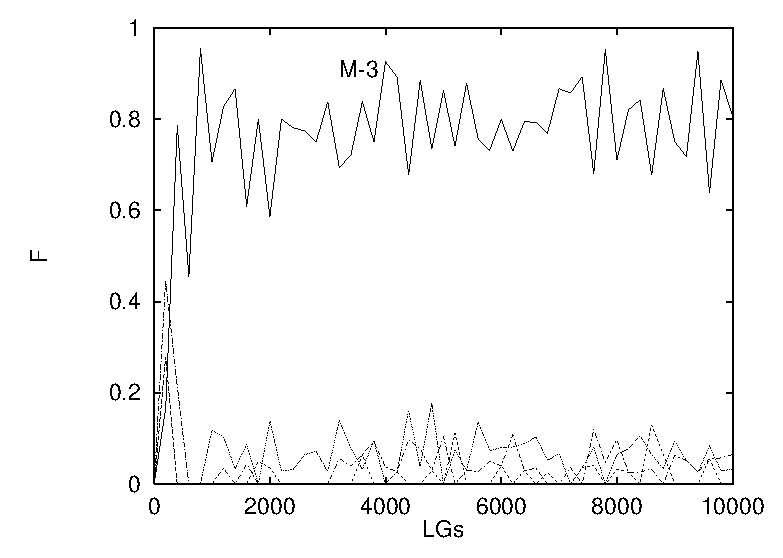
\includegraphics[width=5.5cm]{optimal/rc1-3oli.eps}}
\caption{Referent-meaning competition for L2 and L3 of robots r0 and r1.}
\label{f:opt:rcoli}
\end{figure}

\begin{figure}[t]
\centering
\subfigure[M12]{\includegraphics[width=5.5cm]{optimal/cf0-12oli.eps}}
\subfigure[M28]{\includegraphics[width=5.5cm]{optimal/cf0-28oli.eps}}
\subfigure[M36]{\includegraphics[width=5.5cm]{optimal/cf0-36oli.eps}}
\subfigure[keni]{\includegraphics[width=5.5cm]{optimal/fc0-2oli.eps}}
\caption{Meaning-form competition of robot r0 for (a) M-12, (b) M-28 and (c) M-36. Figure (d) shows the form-meaning competition of {\bf keni}.}
\label{f:opt:cfoli}
\end{figure}


Another striking observation when comparing the competition of this experiment with the competition in the guessing games is that at the bottom there is more and stronger competition here, compare e.g. figures \ref{f:opt:ggcomp2} (a) and \ref{f:opt:rfoli}. Apparently, the observational game strategy is pretty well at developing a coherent lexicon, however the lack of directive feedback allows quite some synonymy. \index{synonymy}

So, although the update principle of the scores works relatively good (conform the naming of referents L0 and L1), the system still allows both many-to-many relations at each level of comparison, except between meaning and referent, which is almost one-to-one. Recall that the association scores are updated according to an association's use, since the robots consider themselves to be successful whenever they communicated an association. Apparently the use alone cannot disambiguate very strong competitions that are structurally present in the communication. \index{polysemy}\index{synonymy}
\index{joint attention|)}
\index{observational game|)}

\section{Summary}

In this chapter the experiment has optimised two games: the guessing game and the observational game. Several parameters and methods that were found to improve the system in the previous chapter were combined in these experiments.

The optimised experiments revealed that the robots are well capable of developing an ontology and lexicon by which they can communicate pretty well. The important features of the optimised experiment are: (1) using new gearing, (2) adopting word-forms additionally when the robots misidentified the topic, (3) a different learning rate and (4) a higher creation probability. 

Further it has been shown that the robots learn the communication system almost up to its potential when they play an observational language game, a result that is not yet reached in the guessing game. 

Establishing joint attention prior to the linguistic communication, however, has a cost. The lexicons that emerge under this condition show a higher level of synonymy. It seems that the pressure to disambiguate is too small because the joint attention makes communication more or less redundant. 

The results of the experiments reported here shall be discussed more thoroughly in the next chapter.


